\documentclass[border=5pt]{standalone}
\usepackage[T1]{fontenc}
\usepackage{lmodern}
\usepackage{pgfplots}
\usepgfplotslibrary{groupplots}
\pgfplotsset{compat=1.18}
\begin{document}
\sffamily
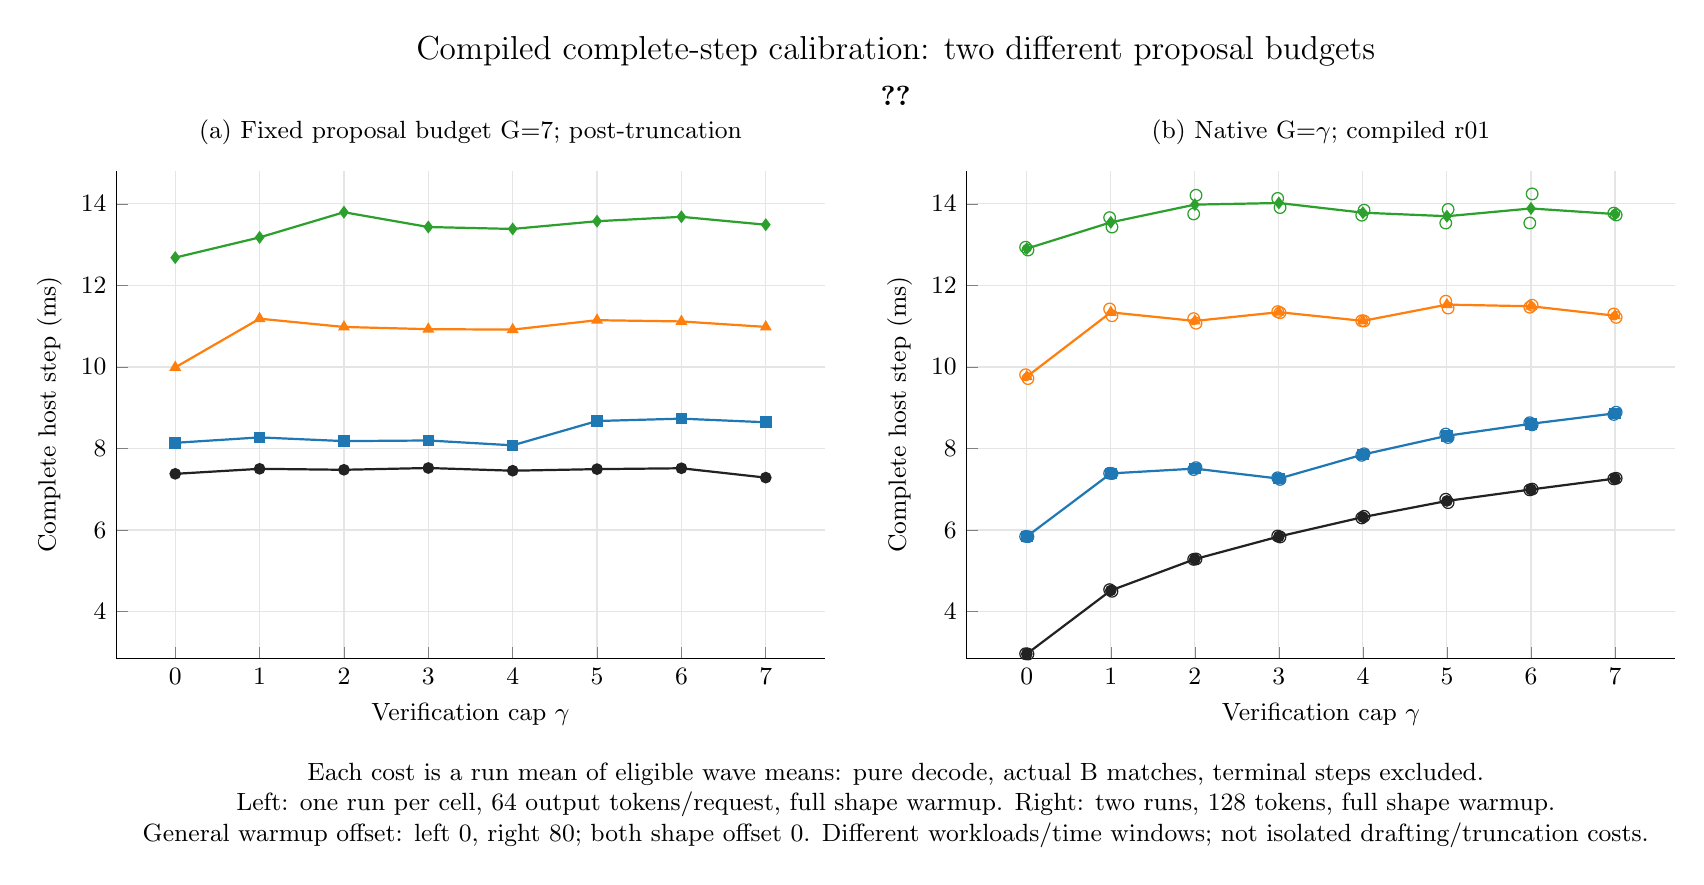
\begin{tikzpicture}
\definecolor{series0}{HTML}{222222}
\definecolor{series1}{HTML}{1f77b4}
\definecolor{series2}{HTML}{ff7f0e}
\definecolor{series3}{HTML}{2ca02c}
\definecolor{series4}{HTML}{d62728}
\definecolor{series5}{HTML}{9467bd}
\definecolor{series6}{HTML}{8c564b}
\definecolor{series7}{HTML}{e377c2}
\begin{groupplot}[group style={group size=2 by 1,horizontal sep=1.8cm},width=9.0cm,height=6.2cm,scale only axis,grid=major,grid style={gray!20},axis lines*=left,tick label style={font=\small},label style={font=\small},title style={font=\small},unbounded coords=jump,ymin=2.8385571413095234,ymax=14.815813648]
\nextgroupplot[title={(a) Fixed proposal budget G=7; post-truncation},xlabel={Verification cap $\gamma$},ylabel={Complete host step (ms)},xtick={0,1,2,3,4,5,6,7},xticklabels={0,1,2,3,4,5,6,7},scaled y ticks=false,yticklabel style={/pgf/number format/fixed,/pgf/number format/precision=2},legend columns=4,legend to name=sharedlegend,legend style={draw=none,font=\small,/tikz/every even column/.append style={column sep=8pt}}]
\addplot+[color=series0,mark=*,mark size=1.7pt,mark options={fill=series0,draw=series0},line width=0.8pt] coordinates {(0,7.37812084476) (1,7.50117768616) (2,7.47731434514) (3,7.52107925293) (4,7.45480315462) (5,7.49357193577) (6,7.51466576344) (7,7.28502890171)};
\addlegendentry{B=1}
\addplot+[only marks,forget plot,color=series0,mark=o,mark size=2.1pt,mark options={fill=white,line width=0.45pt}] coordinates {};
\addplot+[color=series1,mark=square*,mark size=1.7pt,mark options={fill=series1,draw=series1},line width=0.8pt] coordinates {(0,8.13906715827) (1,8.27214199008) (2,8.18095679676) (3,8.19628475221) (4,8.07765106146) (5,8.67399539338) (6,8.73223669568) (7,8.64310516809)};
\addlegendentry{B=4}
\addplot+[only marks,forget plot,color=series1,mark=o,mark size=2.1pt,mark options={fill=white,line width=0.45pt}] coordinates {};
\addplot+[color=series2,mark=triangle*,mark size=1.7pt,mark options={fill=series2,draw=series2},line width=0.8pt] coordinates {(0,9.98901817742) (1,11.1844562659) (2,10.9814263998) (3,10.9273989062) (4,10.9168027695) (5,11.1476579391) (6,11.1170640604) (7,10.9828119625)};
\addlegendentry{B=16}
\addplot+[only marks,forget plot,color=series2,mark=o,mark size=2.1pt,mark options={fill=white,line width=0.45pt}] coordinates {};
\addplot+[color=series3,mark=diamond*,mark size=1.7pt,mark options={fill=series3,draw=series3},line width=0.8pt] coordinates {(0,12.6831205806) (1,13.1784726818) (2,13.7965300256) (3,13.4333407879) (4,13.3862070968) (5,13.575823129) (6,13.6839130625) (7,13.4894583548)};
\addlegendentry{B=64}
\addplot+[only marks,forget plot,color=series3,mark=o,mark size=2.1pt,mark options={fill=white,line width=0.45pt}] coordinates {};
\nextgroupplot[title={(b) Native G=$\gamma$; compiled r01},xlabel={Verification cap $\gamma$},ylabel={Complete host step (ms)},xtick={0,1,2,3,4,5,6,7},xticklabels={0,1,2,3,4,5,6,7},scaled y ticks=false,yticklabel style={/pgf/number format/fixed,/pgf/number format/precision=2}]
\addplot+[color=series0,mark=*,mark size=1.7pt,mark options={fill=series0,draw=series0},line width=0.8pt] coordinates {(0,2.96055796348) (1,4.51648304144) (2,5.2848314198) (3,5.84079759084) (4,6.31612819784) (5,6.71284544655) (6,6.99419195972) (7,7.26196628498)};
\addplot+[only marks,forget plot,color=series0,mark=o,mark size=2.1pt,mark options={fill=white,line width=0.45pt}] coordinates {(-0.014,2.96428557143) (0.014,2.95683035553) (0.986,4.53659039549) (1.014,4.49637568739) (1.986,5.27996079838) (2.014,5.28970204121) (2.986,5.85241132139) (3.014,5.82918386029) (3.986,6.29661936329) (4.014,6.33563703239) (4.986,6.75409746663) (5.014,6.67159342648) (5.986,6.98529137812) (6.014,7.00309254132) (6.986,7.25480505436) (7.014,7.26912751561)};
\addplot+[color=series1,mark=square*,mark size=1.7pt,mark options={fill=series1,draw=series1},line width=0.8pt] coordinates {(0,5.83975048983) (1,7.38838427895) (2,7.50607529571) (3,7.26101621321) (4,7.85107127035) (5,8.31124670662) (6,8.60599014551) (7,8.86238945378)};
\addplot+[only marks,forget plot,color=series1,mark=o,mark size=2.1pt,mark options={fill=white,line width=0.45pt}] coordinates {(-0.014,5.84260426339) (0.014,5.83689671627) (0.986,7.39231505058) (1.014,7.38445350733) (1.986,7.48254580957) (2.014,7.52960478185) (2.986,7.28110263351) (3.014,7.24092979292) (3.986,7.83216831605) (4.014,7.86997422466) (4.986,8.3537266506) (5.014,8.26876676264) (5.986,8.63195707254) (6.014,8.58002321848) (6.986,8.83524730302) (7.014,8.88953160454)};
\addplot+[color=series2,mark=triangle*,mark size=1.7pt,mark options={fill=series2,draw=series2},line width=0.8pt] coordinates {(0,9.76209465873) (1,11.3397461714) (2,11.1292324888) (3,11.3446431439) (4,11.1308288253) (5,11.5293166688) (6,11.489553681) (7,11.2582347972)};
\addplot+[only marks,forget plot,color=series2,mark=o,mark size=2.1pt,mark options={fill=white,line width=0.45pt}] coordinates {(-0.014,9.80902835119) (0.014,9.71516096627) (0.986,11.4225755815) (1.014,11.2569167612) (1.986,11.185665594) (2.014,11.0727993836) (2.986,11.3578251229) (3.014,11.331461165) (3.986,11.1343652216) (4.014,11.127292429) (4.986,11.6137748451) (5.014,11.4448584925) (5.986,11.4657226294) (6.014,11.5133847325) (6.986,11.2999540273) (7.014,11.2165155671)};
\addplot+[color=series3,mark=diamond*,mark size=1.7pt,mark options={fill=series3,draw=series3},line width=0.8pt] coordinates {(0,12.9034215992) (1,13.5479965739) (2,13.9833216299) (3,14.0227825205) (4,13.7852829853) (5,13.6985607348) (6,13.8885840923) (7,13.7515447344)};
\addplot+[only marks,forget plot,color=series3,mark=o,mark size=2.1pt,mark options={fill=white,line width=0.45pt}] coordinates {(-0.014,12.9378319444) (0.014,12.869011254) (0.986,13.6639099886) (1.014,13.4320831591) (1.986,13.754359026) (2.014,14.2122842338) (2.986,14.1351702055) (3.014,13.9103948356) (3.986,13.7232000588) (4.014,13.8473659118) (4.986,13.5308362273) (5.014,13.8662852424) (5.986,13.5311935231) (6.014,14.2459746615) (6.986,13.7744437812) (7.014,13.7286456875)};
\end{groupplot}
\path (group c1r1.north west) -- node[above=1.2cm,font=\large] {Compiled complete-step calibration: two different proposal budgets} (group c2r1.north east);
\path (group c1r1.north west) -- node[above=0.7cm] {\ref{sharedlegend}} (group c2r1.north east);
\path (group c1r1.south west) -- node[below=1.2cm,align=center,font=\small] {Each cost is a run mean of eligible wave means: pure decode, actual B matches, terminal steps excluded.\\Left: one run per cell, 64 output tokens/request, full shape warmup. Right: two runs, 128 tokens, full shape warmup.\\General warmup offset: left 0, right 80; both shape offset 0. Different workloads/time windows; not isolated drafting/truncation costs.} (group c2r1.south east);
\end{tikzpicture}
\end{document}
